\subsection{Predicate tree}
\label{sec:PredicateTree}
In this section, we will answer the question ``how to build a tree for a predicate in RFuzzy Program". For convenience, we call the corresponding tree for the predicate as \textit{predicate tree}. We start by transforming a RFuzzy Program, to obtain the subset of program which we use to create predicate tree in section \ref{sec:TransformRFuzzy}. The approach of constructing predicate trees from subset of program is presented in section \ref{sec:Construct}. In order to compare two predicate trees, the structure of them should be the same, and also preserve the embedded meanings. For this, the concept ``equivalent trees" is introduced in section \ref{sec:EquivalentTree}. According to ``equivalent trees", the predicate tree could be constructed with \textit{identities}, which maintain the semantic meaning but reform the structure. It is described in section \ref{sec:ReConstruct}.

\subsubsection{Transform RFuzzy program}
\label{sec:TransformRFuzzy}
In a \textit{RFuzzy program} $P=(R,D,T)$, $R$ is a set of \textit{fuzzy clauses}, $D$ is a set of \textit{default value declarations} and $T$ is a set of \textit{type declarations}. In order to construct a tree for each predicate in $P$, we need to filter and reform some parts of $P$. This procedure is called \textit{transformation}, in which two steps are taken, one is filtering and the other is reforming. In this section, the details \textit{how} and \textit{why} are presented. 

The result of first step \textit{filtering} is a tuple $P'=(R',D',T')$, which is generated from $P$ by following constrains,
\begin{enumerate}
 \item Refined $R'$

    $R$ as a set of \textit{fuzzy clauses}, includes fuzzy clauses, which are written as, \[A \stackrel{c,F_c}{\longleftarrow}F(B_1,...,B_n)\]
    where $A \in TB_{\Pi,\Sigma,V}$ is called the head, $B_1,...,B_n \in TB_{\Pi,\Sigma,V}$ is called the body, $c\in[0,1]$ is the credibility value, and $F_c\in\{\&_1,...,\&_k\}\subset\Omega^{(2)}$ and $F\in\Omega^{(n)}$ are connectives symbols. $F_c$ is to combine the credibility of the rule and the truth value of the body. $F$ is to combine the truth values of the subgoals in the body.
   
    A \textit{fuzzy fact} is a special case where $c=1$, $F_c$ is the usual product of real numbers  `` . ''  , $n=0$, $F\in\Omega^{(0)}$. It is written as \[A \longleftarrow v\]
    where $c$ and $F_c$ are omit. 

    The similarity between predicates is a relevant value of comparison between two predicates, rather than the absolute value described in \textit{fuzzy facts}. Therefore, \textit{fuzzy facts} will be out of consideration of similarity between predicates.
    
    Thus, $R'$ is a set of all \textit{fuzzy clauses}, but not \textit{fuzzy facts}, notated as, $R'=R\backslash R_{facts}$.
 \item Refined $D'$

    A \textit{default value declaration} for a predicate $p \in \Pi ^{(n)}$ is written as 
    \begin{center}
       $default(p/n)=[\delta_1$ if $\varphi_1$, ..., $\delta_m$ if $\varphi_m]$
    \end{center}
    where $\delta_i\in[0,1]$ for all $i$. The $\varphi_i$ are first-order formulas restricted to terms in $p$ from $TU_{\Sigma,V_p}$, the predicates $=$ and $\neq$, the symbol true and the junctors $\wedge$ and $\vee$ in their usual meaning, which are \textit{`and'}, \textit{ `or'}.

    There is a special case called \textit{unconditional} default value declaration where $m=1$ and $\varphi_1=true$ in the default value declarations. In this case, the predicate $p/n$ will not be related to any other predicates, therefore, it is out of consideration of similarity.

    Thus, $D'$ is all the \textit{conditional} default value declarations, notated as, $D'=D\backslash D_{unconditional}$.

 \item Refined $T'$
    
    \[T=T_{term} \cup T_{predicate}\]
    $T_{term}$ is a set of all \textit{term type declarations}, which assign a type $\tau \in \mathcal{T}$ to a term $t \in \mathbb{HU}$ and is written as $t : \tau$. $T_{predicate}$ is a set of all predicate type declarations. A \textit{predicate type declaration} assigns a type $(\tau_1,...,\tau_n) \in \mathcal{T}^n$ to predicate $p\in\Pi^n$ and is written as $p : (\tau_1,...,\tau_n)$, where $\tau_i$ is the type of $p$'s $i$-th argument.

    The $T_{term}$ is not related to predicates at all, so it will not be taken into account of the similarity between predicates.

    Therefore, $T'=T_{predicate}$.
 \end{enumerate}

After filtering the RFuzzy program $P=(R,D,T)$ into $P'=(R',D',T')$, the second step is taken to reform $D'$ into $D_{new}$. A \textit{default value declarations} in $D'$ is
\begin{center}
 $default(p/n)=[\delta_1$ if $\varphi_1$,..., $\delta_m$ if $\varphi_m]$ 
\end{center}

Since $\varphi_i$ are FOL formulas, it always could be in a DNF(Disjunctive Normal Form), $\varphi_i^1 \vee ... \vee \varphi_i^{k_i}$, then $default(p/n) = \delta_i$ if $\varphi_i$ is written in the \textit{fuzzy clauses} format $A \stackrel{c,F_c}{\longleftarrow}F(B_1,...,B_n)$.

\[p(\vec{x}) \stackrel{\delta_i,.}{\longleftarrow} \varphi_i^1\]
\[\vdots\]
\[p(\vec{x}) \stackrel{\delta_i,.}{\longleftarrow} \varphi_i^{k_i}\]

Then $default(p/n)=[\delta_1$ if $\varphi_1$,..., $\delta_m$ if $\varphi_m]$ could be reformed as,

\[p(\vec{x}) \stackrel{\delta_1,.}{\longleftarrow} \varphi_1^1\]
\[\vdots\]
\[p(\vec{x}) \stackrel{\delta_1,.}{\longleftarrow} \varphi_1^{k_1}\]
\[\vdots\]
\[p(\vec{x}) \stackrel{\delta_m,.}{\longleftarrow} \varphi_m^1\]
\[\vdots\]
\[p(\vec{x}) \stackrel{\delta_m,.}{\longleftarrow} \varphi_m^{k_m}\]

Apparently, the reforming procedure from $D'$ into $D_{new}$ preserves the semantic equivalence. The result of \textit{reforming} functioning over $P'$ is $P_{new}=(R_{new},T_{new})$, where $R_{new} = R' \cup D_{new}$ a union of the \textit{fuzzy clauses} and \textit{default value declarations} in the same form of \textit{fuzzy clauses}'s, $T_{new}=T'$. 

\subsubsection{Constructing the predicate tree}
\label{sec:Construct}
Every predicate in the \textit{fuzzy program} $P_{new}$ could be represented as a tree. A formal description of the approach of generating a corresponding tree for a certain predicate begins with the definition of \textit{atomic predicate} and \textit{complex predicate}.
 
\begin{defin}\textbf{(Atomic predicate)}.
Predicates appearing only in the bodies of rules in $R_{new}$, and never appearing in the heads of any rules, are \textbf{atomic predicates}, since they are not defined by any other predicates.  
\end{defin}

\begin{defin}\textbf{(Complex predicate)}.
Predicates appearing in the heads of rules in $R_{new}$ are \textbf{complex predicates}, in the sense that they could be represented by the bodies of the rules with them as heads. 
\end{defin}

\textit{Atomic predicate} is written as $p_{a}$, and \textit{complex predicate} as $p_{c}$. \textit{Atomic predicate} $p_{a}$ is represented in a tree-form, which is a node with information $\tau_{p_{a}}$, and without any children nodes, where $\tau_{p_{a}}$ is the \textit{type} of $p_{a}$. \textit{Complex predicate} $p_{c}$ by definition must appear in the head of some rules in $P_{new}$, whose form is,
\[p_{c}(\vec{t}) \stackrel{c,F_c}{\longleftarrow}F(p_1(\vec{t_1}),...,p_n(\vec{t_n}))\] 
Then the tree of $p_{c}$ has a root $N_{p_{c}}$, with its node information, $c$, $F_c$, $F$, and $\tau_{p_{c}}$, which is the \textit{type} of $p_{c}$. The branches from $N_{p_{c}}$ are $N_{p_1}$, ..., $N_{p_n}$, which are expanded as corresponding trees recursively. Thus, the leaves in the tree are \textit{atomic predicates}, which never appear in the heads of any rules in $R_{new}$, and can not be expanded any more.

If there are several rules defining a certain predicate $p$, then there are different corresponding trees for $p$, since the expanding procedure is recursive, which means, the children of $p$ node could also be defined in several other rules, then more possible trees are generated. 

%\newpage
\begin{figure}[t]
\begin{center}
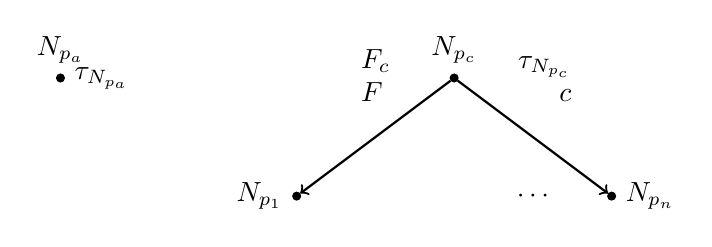
\begin{tikzpicture}[yscale=-1,
place/.style={circle,draw=black, fill=black, inner sep=0pt, 
              minimum size=1mm}]

 \node[place] (1st) at (1, 0) [label=above: $N_{p_{a}}$,
                               label=right: $\tau_{N_{p_{a}}}$] {};
	

\begin{scope}[xshift=4cm]
  \node[place] (1st) at (2, 0) [label=above: $N_{p_{c}}$,
                                label=right: 
       \begin{tabular}{l r}
         & $\tau_{N_{p_{c}}}$ \\
         & $c$\\
       \end{tabular},
       label=left:
       \begin{tabular}{l l}
         $F_c$ &\\
         $F$ &\\
       \end{tabular}] {};
  \node[place] (2nd) at (0, 1.5) [label=left: $N_{p_1}$] {};
  \node[place] (3rd) at (4, 1.5) [label=right: $N_{p_n}$]{}; 

  \node (dots) at (3,1.5) {$\cdots$};
	
  \draw[->, thick] (1st) -- (2nd);
  \draw[->, thick] (1st) -- (3rd);
\end{scope}

\end{tikzpicture}
\caption{Predicate Tree}
\label{Predicate Tree}
\end{center}   
\end{figure}

% pictures

\begin{ex}\label{ConstructPredicateTree}
Here is a part of short RFuzzy program,
\begin{center}
\begin{tabular}{l l}
$has\_tasty\_food:$  & $(Restaurant)$\\

$has\_healthy\_food:$ &  $(Restaurant)$\\

$has\_good\_service:$  & $(Restaurant)$\\

$tasty\_restaurant:$  & $(Restaurant)$\\

$good\_restaurant:$  & $(Restaurant)$\\
\end{tabular}
\end{center}
\begin{tabular}{l l l}
$tasty\_restaurant(X)$ & $\stackrel{1.0,.}{\longleftarrow} prod$ & $has\_tasty\_food(X)$\\

$good\_restaurant(X)$ & $\stackrel{0.8,.}{\longleftarrow} prod$ & $has\_healthy\_food(X), has\_good\_service(X)$ \\

\end{tabular}
\[Sim(has\_healthy\_food, has\_tasty\_food) = 0.6\]
\end{ex}

The corresponding trees for atomic predicates $has\_tasty\_food$,
$has\_healthy\_food$, \linebreak[4] $has\_good\_service$ are,
\begin{center}
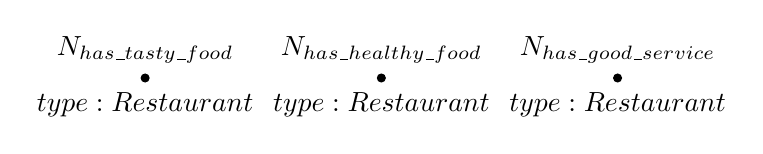
\begin{tikzpicture}[yscale=-1,
place/.style={circle,draw=black, fill=black, inner sep=0pt, 
              minimum size=1mm}]

 \node[place] (1st) at (0, 0) [label=above: $N_{has\_tasty\_food}$,
                               label=below: $type : Restaurant$] {};
	

\begin{scope}[xshift=3cm]
  \node[place] (1st) at (0, 0) [label=above: $N_{has\_healthy\_food}$,
                               label=below: $type : Restaurant$] {};
\end{scope}

\begin{scope}[xshift=6cm]
  \node[place] (1st) at (0, 0) [label=above: $N_{has\_good\_service}$,
                               label=below: $type : Restaurant$] {};
\end{scope}

\end{tikzpicture}
\end{center}   
The corresponding tree for complex predicate $tasty\_restaurant$ is,
\begin{center}
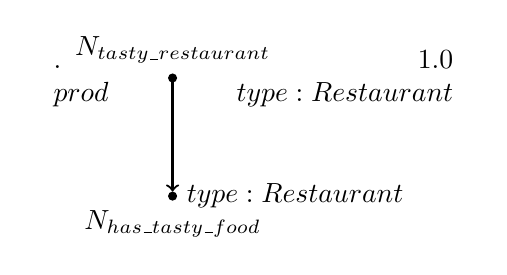
\begin{tikzpicture}[yscale=-1,
place/.style={circle,draw=black, fill=black, inner sep=0pt, 
              minimum size=1mm}]

 \node[place] (1st) at (0, 0) [label=above: $N_{tasty\_restaurant}$,
                                label=right: 
       \begin{tabular}{l r}
         & $1.0$\\
         & $type : Restaurant$ \\
       \end{tabular},
       label=left:
       \begin{tabular}{l l}
         $.$ &\\
         $prod$ &\\
       \end{tabular}] {};
  \node[place] (2nd) at (0, 1.5) [label=below: $N_{has\_tasty\_food}$,
                                  label=right: $type : Restaurant$] {};
 
  \draw[->, thick] (1st) -- (2nd);

\end{tikzpicture}
\end{center}   
The corresponding tree for complex predicate $good\_restaurant$ is,
\begin{center}
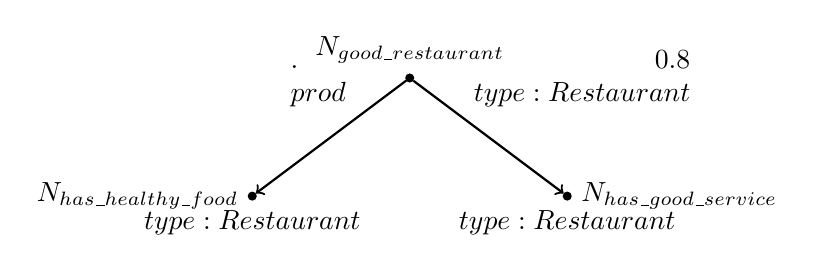
\begin{tikzpicture}[yscale=-1,
place/.style={circle,draw=black, fill=black, inner sep=0pt, 
              minimum size=1mm}]

  \node[place] (1st) at (2, 0) [label=above: $N_{good\_restaurant}$,
                                label=right: 
       \begin{tabular}{l r}
         & $0.8$\\
         & $type : Restaurant$ \\
       \end{tabular},
       label=left:
       \begin{tabular}{l l}
         $.$ &\\
         $prod$ &\\
       \end{tabular}] {};
  \node[place] (2nd) at (0, 1.5) [label=left: $N_{has\_healthy\_food}$,
                                  label=below: $type : Restaurant$] {};
  \node[place] (3rd) at (4, 1.5) [label=right: $N_{has\_good\_service}$,
                                  label=below: $type : Restaurant$]{}; 

  \draw[->, thick] (1st) -- (2nd);
  \draw[->, thick] (1st) -- (3rd);

\end{tikzpicture}
\end{center}   


\begin{comment}
\begin{prop} \textbf{Number of corresponding tree for predicate $p$}
The number of the corresponding trees for each predicate is exponential over the number of rules $n$.
\end{prop}

Let $P$ be a RFuzzy program, it has rules in the following form,
\[p() :- p_1(\vec{X})\]
\[p_1(\vec{X}) :- p_{11}(\vec{X})\]
\[p_1(\vec{X}) :- p_{12}(\vec{X})\]
\[p_{11}(\vec{X}) :- p_{111}(\vec{X})\]
\[p_{11}(\vec{X}) :- p_{112}(\vec{X})\]
\[p_{12}(\vec{X}) :- p_{121}(\vec{X})\]
\[p_{12}(\vec{X}) :- p_{122}(\vec{X})\]
\[\vdots\]
continue, for each predicate $p_{i}$, there are two rules defining it, in each rule, there is only one atom in the body.

Suppose that there is $n$ rules in $P$, and the number of trees could be generated for predicate $p$ is $2^{n/2}$, which is exponential of n. However, practically, the number of corresponding trees for certain predicate will not achieve the exponential, since the rules will be defined more reasonable, rather than the given example.

In order to retrieve the similarity between two predicates, creating all their corresponding trees is not optimal approach, considering the possible exponential explosion.  Therefore, there is a more efficient algorithm is proposed in the following sections.  

\end{comment}
\subsubsection{Equivalence between predicate trees}
\label{sec:EquivalentTree}
In order to compare two predicate trees with different number of children, we reconstruct them with the same number of children, preserving the original semantic meaning. For this, the concept ``equivalent tree" is introduced in this section.

For each rule in $P_{new}$ that $A \stackrel{c,F_c}{\longleftarrow}F(B_1,...,B_n)$, under its interpretations, it is viewed as a function in the following form,
\[A^{\mathcal{I}} = OP (c,B_1^{\mathcal{I}},...,B_n^{\mathcal{I}})\]
where $OP=(\hat{F_c},\hat{F})$ is a pair, representing the operations over \textit{credit value} $c$, and other interpretation over atoms $B_i$ in the body of the rule. 

\begin{defin}\textbf{(Identity for complex predicate).}
\label{def:IdentityComplex}
 There exists a formula $\alpha$ under the operations of RFuzzy Program, which makes
 \begin{equation}\label{eq:equivalentFormula}
 OP(c,B_1^{\mathcal{I}},...,B_n^{\mathcal{I}},\alpha^{\mathcal{I}})=OP(c,B_1^{\mathcal{I}},...,B_n^{\mathcal{I}})
 \end{equation}
for each interpretation $\mathcal{I}$. Therefore, the formula $\alpha$ is called \textit{identity} for $OP$. The existence of $\alpha$ depends on the operation $OP$.
\end{defin}

If \textit{identity} $\alpha$ exists for some $OP$, then the rule
\begin{center}
\begin{equation}\label{eq:orginalRule}
A \stackrel{c,F_c}{\longleftarrow}F(B_1,...,B_n)
\end{equation}
\end{center}
could be rewritten as
\begin{center}
\begin{equation}\label{eq:equivalentRule}
A \stackrel{c,F_c}{\longleftarrow}F(B_1,...,B_n,\alpha,...,\alpha)
\end{equation}
\end{center}

Since the procedure of rewriting preserves the semantic equivalence, the corresponding trees of rules \ref{eq:orginalRule} and \ref{eq:equivalentRule} represent the same semantic meaning.

\begin{defin} \textbf{(Identity for atomic predicate).}
\label{def:IdentityAtomic}
For some certain $OP=(\hat{F_c},\hat{F})$, there exists a formula $\beta$ under the operations of RFuzzy Program, which makes,
\[A^{\mathcal{I}} = OP(c,A^{\mathcal{I}},\beta^{\mathcal{I}})\]
for any interpretation $\mathcal{I}$, where $c$ is a real number in the range of $[0,1]$. Therefore, $\beta$ is called identity for $OP$.
\end{defin}

We are going to show the existence of identity for any $OP=(\hat{F_c},\hat{F})$ here. In mathematical logic, there are several formal systems of \textit{Fuzzy Logic}, and most of them belong to so-called \textit{t-norm fuzzy logics} \cite{HP98}.
A t-norm abbreviated of \textit{triangular norm} is a binary algebraic operation on the interval [0, 1], which is use to generalize conjunction in t-norm fuzzy logic. A t-norm \cite{KPMRPE00} is defined as a function $\top: [0, 1]\times[0, 1]\rightarrow[0, 1]$, which satisfies the following properties:
\begin{itemize}
\item Commutativity: $\top(a, b) = \top(b, a)$
\item Monotonicity: $\top(a, b) \leq \top(c, d)$ if $a \leq c$ and $b \leq d$
\item Associativity: $\top(a, \top(b, c)) = \top(\top(a, b), c)$
\item Identity element: $\top(a, 1) = a$
\end{itemize}

T-conorm (S-norm) is dual to t-norm under the order-reversing operation which assigns 1-x to x on [0, 1]. Given a t-norm, the complementary t-conorm is defined by
\[\bot(a,b) = 1- \top(1-a,1-b)\]
A t-conorm is used to represent logical disjunction in t-norm fuzzy logic. It satisfies the following conditions, which can be used for an equivalent axiomatic definition of t-conorm independently of t-norm:
\begin{itemize}
\item Commutativity: $\bot(a, b) = \bot(b, a)$
\item Monotonicity: $\bot(a, b) \leq \bot(c, d)$ if $a \leq c$ and $b \leq d$
\item Associativity: $\bot(a, \bot(b, c)) = \bot(\bot(a, b), c)$
\item Identity element: $\bot(a, 0) = a$
\end{itemize}

$\hat{F_c}$ and $\hat{F}$  are the truth functions of many-valued connectives $F_c$ and $F$ respectively. They are defined by t-norm or t-conorm. It implies that for any $\hat{F_c}$ or $\hat{F}$, there exists an identity, since a t-norm and a t-conorm has $1$ and $0$ as their identities respectively. Taking Lukasiewicz logic \cite{L20} as an instance, which is one of t-norm fuzzy logics originally defined in the early 20th-century by Jan Lukasiewicz. The connectives and their functions are shown below.
\begin{itemize}
\item Implication: $F_{\rightarrow}(x,y) = min\{1,1-x+y\}$
\item Equivalence: $F_{\leftrightarrow}(x,y) = 1-\lvert x-y \rvert$
\item Negation:  $F_{\neg}(x) = 1-x$
\item Weak Conjunction: $F_{\wedge}(x,y)=min\{x,y\}$
\item Weak Disjunction:  $F_{\vee}(x,y)=max\{x,y\}$
\item Strong Conjunction: $F_{\otimes}(x,y)=max\{0,x+y-1\}$
\item Strong Disjunction:   $F_{\oplus}(x,y)=min\{1,x+y\}$
\end{itemize}
The connectives defined by t-norm are Equivalence, Weak Conjunction, Strong Disjunction, which have $1$ as their identities. Implication, Weak Disjunction, Strong Conjunction are defined by t-conorm and $0$ is the identity.

For example, $F_{\rightarrow}(x,y) = F_{\rightarrow}(F_{\rightarrow}(x,y),1)$, if we use $F_{\rightarrow}$ to represent implication with arbitrary arguments, then $F_{\rightarrow}(x,y) = F_{\rightarrow}(x,y,1)$, which satisfies formula \ref{eq:equivalentFormula} in definition \ref{def:IdentityComplex}.






\subsubsection{Reconstructing predicate trees with equivalence}
\label{sec:ReConstruct}
In this section, the approach of constructing predicates tree with equivalence is displayed, which is used for expanding two comparing nodes with the same structure in the algorithm introduced in section \ref{sec:Algorithm}.

%\begin{center}
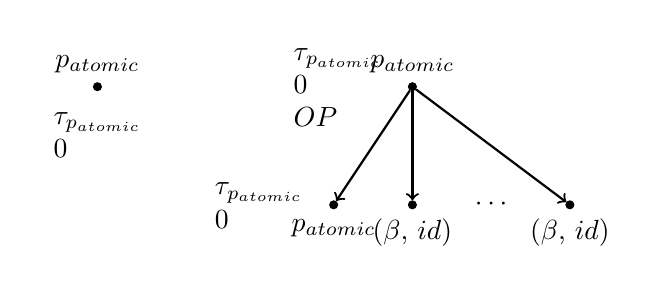
\begin{tikzpicture}[yscale=-1,
place/.style={circle,draw=black, fill=black, inner sep=0pt, 
              minimum size=1mm}]

	\node[place] (1st) at (1, 0) [label=above: $p_{atomic}$,
                                      label=below:
            \begin{tabular}{l}
              $\tau_{p_{atomic}}$\\
              $0$\\
            \end{tabular}] {};

\begin{scope}[xshift=4cm]
  \node[place] (1st) at (1, 0) [label=above: $p_{atomic}$,
                                label=left: 
             \begin{tabular}{l}
              $\tau_{p_{atomic}}$\\
              $0$\\
              $OP$\\ 
             \end{tabular}
] {};
	\node[place] (2nd) at (0, 1.5) [label=below: $p_{atomic}$,
                                        label=left: 
             \begin{tabular}{l}
              $\tau_{p_{atomic}}$ \\
              $0$ \\
             \end{tabular}
]{};
        \node[place] (3rd) at (1, 1.5) [label=below: {($\beta$, $id$)}] {};
	\node[place] (4rd) at (3, 1.5) [label=below: {($\beta$, $id$)}] {}; 

	\node (dots) at (2,1.5) {$\cdots$};
	
	\draw[->, thick] (1st) -- (2nd);
	\draw[->, thick] (1st) -- (3rd);
        \draw[->, thick] (1st) -- (4rd);
\end{scope}


\end{tikzpicture}
\end{center}   

\begin{itemize}
 \item \textit{Atomic predicate}

Suppose that $p_a$ is a \textit{atomic predicate}. Its type is $\tau$. The identity for some $OP$ associated with $p_a$ is $\beta$. 

The corresponding tree of it is a node $N_{p_a}$ with information, which are $\tau$ of $p_a$ and a number $0$, indicating that $p_a$ is atomic predicate. There are no branches for the node $N_{p_a}$. 

With the equivalence extension, the corresponding tree is presented in figure \ref{fig:APT}. The root is a node $N_{p_a}$ with information, which are the \textit{type} of $p_a$ $\tau$, the operation $OP$ and atomic mark $0$. The branches are a node $N'_{p_a}$ and several nodes $N_{\beta}$.  $N'_{p_a}$ carries information $\tau$, which is $p_a$'s type and atomic mark $0$. $N_{\beta}$ carries information of identity $\beta$ and identity mark $id$, the number of such nodes depends on two comparing predicates.

% pictures
\begin{figure}[h!]
\begin{center}
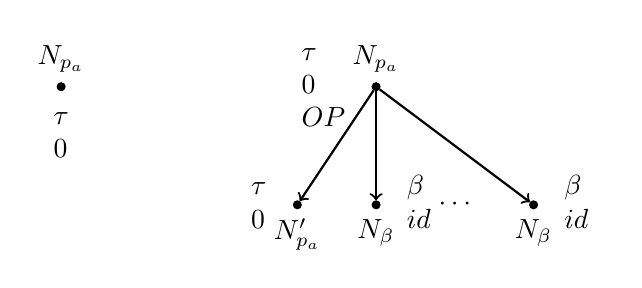
\begin{tikzpicture}[yscale=-1,
place/.style={circle,draw=black, fill=black, inner sep=0pt, 
              minimum size=1mm}]

	\node[place] (1st) at (1, 0) [label=above: $N_{p_a}$,
                                      label=below:
            \begin{tabular}{l}
              $\tau$\\
              $0$\\
            \end{tabular}] {};

\begin{scope}[xshift=4cm]
  \node[place] (1st) at (1, 0) [label=above: $N_{p_a}$,
                                label=left: 
             \begin{tabular}{l}
               $\tau$\\
               $0$\\
               $OP$\\
             \end{tabular}
] {};
	\node[place] (2nd) at (0, 1.5) [label=below: $N'_{p_a}$,
                                        label=left: 
             \begin{tabular}{l}
              $\tau$ \\
              $0$ \\
             \end{tabular}
]{};
        \node[place] (3rd) at (1, 1.5) [label=below: $N_{\beta}$,
        							  label=right: 
             \begin{tabular}{l}
              $\beta$ \\
              $id$ \\
             \end{tabular}        
        ] {};
	\node[place] (4rd) at (3, 1.5) [label=below: $N_{\beta}$,
							  label=right: 
             \begin{tabular}{l}
              $\beta$ \\
              $id$ \\
             \end{tabular}
	] {}; 

	\node (dots) at (2,1.5) {$\cdots$};
	
	\draw[->, thick] (1st) -- (2nd);
	\draw[->, thick] (1st) -- (3rd);
         \draw[->, thick] (1st) -- (4rd);
\end{scope}


\end{tikzpicture}
\end{center}   
\caption{Atomic predicate tree with equivalence}
\label{fig:APT}
\end{figure}

 \item \textit{Complex predicate}

For \textit{complex predicate}, there would be at least one rule defining it as,
\[p_c(\vec{t}) \stackrel{c,F_c}{\longleftarrow}F(p_1(\vec{t_1}),...,p_n(\vec{t_n}))\]
and for $OP=(\hat{F_c},\hat{F})$, there exists an identity $\alpha$.  $\tau$, and $\tau_{i}$ are represented types of $p_c$ and $p_{i}$ respectively.

The corresponding tree for $p_c$ is

% pciture
\begin{center}
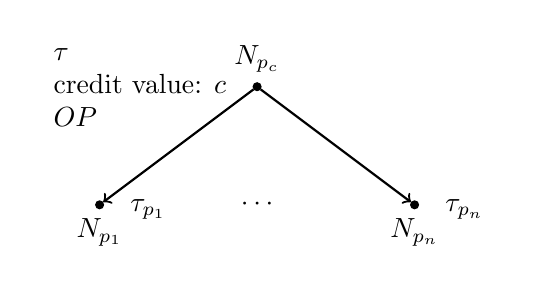
\begin{tikzpicture}[yscale=-1,
place/.style={circle,draw=black, fill=black, inner sep=0pt, 
              minimum size=1mm}]

  \node[place] (1st) at (2, 0) [label=above: $N_{p_c}$,
                                label=left: 
             \begin{tabular}{l}
               $\tau$\\
               credit value: $c$\\
               $OP$\\
             \end{tabular}
] {};
	\node[place] (2nd) at (0, 1.5) [label=below: $N_{p_1}$,
							  label=right: 
             \begin{tabular}{l}
            $\tau_{p_1}$\\
             \end{tabular}
	] {};
        \node[place] (3rd) at (4, 1.5) [label=below: $N_{p_n}$,
        							label=right: 
             \begin{tabular}{l}
             $\tau_{p_n}$ \\
             \end{tabular}        
        ] {}; 
	
	\node (dots) at (2,1.5) {$\cdots$};
	
	\draw[->, thick] (1st) -- (2nd);
	\draw[->, thick] (1st) -- (3rd);
        

\end{tikzpicture}
\end{center}   

where $N_{p_c}$ is the root with information which are $\tau$, $OP$ and credit value $c$. $N_{p_i}$s are the branches carrying their \textit{types} as information.

With the equivalence extension, the tree is 

% pictures
\begin{center}
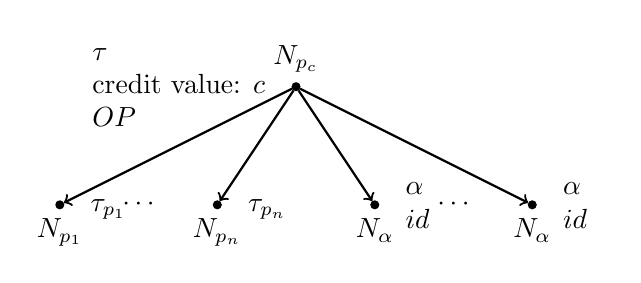
\begin{tikzpicture}[yscale=-1,
place/.style={circle,draw=black, fill=black, inner sep=0pt, 
              minimum size=1mm}]

  \node[place] (1st) at (3, 0) [label=above: $N_{p_c}$,
                                label=left: 
             \begin{tabular}{l}
               $\tau$\\
               credit value: $c$\\
               $OP$\\
             \end{tabular}
] {};
	\node[place] (2nd) at (0, 1.5) [label=below: $N_{p_1}$,
							label=right: 
             \begin{tabular}{l}
            $\tau_{p_1}$\\
             \end{tabular}
	] {};
	\node[place] (3rd) at (2, 1.5) [label=below: $N_{p_n}$,
							  label=right: 
             \begin{tabular}{l}
            $\tau_{p_n}$\\
             \end{tabular}
	] {}; 
        \node[place] (4rd) at (4, 1.5) [label=below: $N_{\alpha}$,
        						  label=right: 
             \begin{tabular}{l}
            $\alpha$\\
            $id$\\
             \end{tabular}
        ] {}; 
        \node[place] (5rd) at (6, 1.5) [label=below: $N_{\alpha}$,
        						  label=right: 
             \begin{tabular}{l}
            $\alpha$\\
            $id$
             \end{tabular}
	] {}; 

	\node (dots) at (1,1.5) {$\cdots$};
        \node (dots) at (5,1.5) {$\cdots$};
	
	\draw[->, thick] (1st) -- (2nd);
	\draw[->, thick] (1st) -- (3rd);
        \draw[->, thick] (1st) -- (4rd);
        \draw[->, thick] (1st) -- (5rd);
\end{tikzpicture}
\end{center}   
 $N_{p_c}$ is the root with information which are $\tau$, $OP$ and credit value $c$. $N_{p_i}$s are the branches with their \textit{types} as information, and several nodes $N_{\alpha}$ carrying information of identities $\alpha$ with identity mark $id$ are added as extra branches depending on two comparing predicates.
\end{itemize}

\begin{ex}
Continuation of the example \ref{ConstructPredicateTree}, reconstruct predicate trees with equivalence.

\begin{center}
\begin{tabular}{l l}
$has\_tasty\_food:$  & $(Restaurant)$\\

$has\_healthy\_food:$ &  $(Restaurant)$\\

$has\_good\_service:$  & $(Restaurant)$\\

$tasty\_restaurant:$  & $(Restaurant)$\\

$good\_restaurant:$  & $(Restaurant)$\\
\end{tabular}
\end{center}
\begin{tabular}{l l l}
$tasty\_restaurant(X)$ & $\stackrel{1.0,.}{\longleftarrow} prod$ & $has\_tasty\_food(X)$\\

$good\_restaurant(X)$ & $\stackrel{0.8,.}{\longleftarrow} prod$ & $has\_healthy\_food(X), has\_good\_service(X)$ \\
\end{tabular}

The predicate tree for \textit{has\_tasty\_food} is represented in figure \ref{fig:ex1}.
\begin{figure}[h!]
\begin{center}
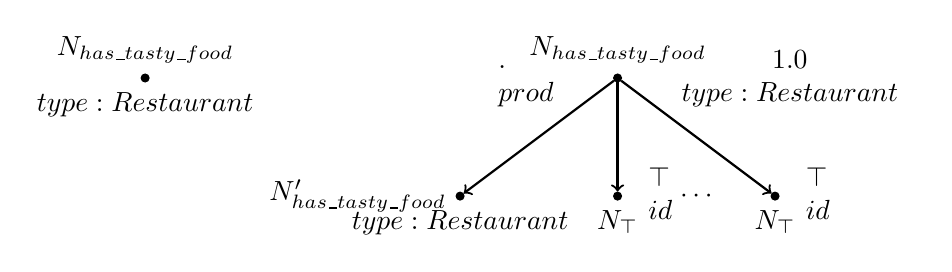
\begin{tikzpicture}[yscale=-1,
place/.style={circle,draw=black, fill=black, inner sep=0pt, 
              minimum size=1mm}]

 \node[place] (1st) at (0, 0) [label=above: $N_{has\_tasty\_food}$,
                               label=below: $type : Restaurant$] {};
	

\begin{scope}[xshift=4cm]
  \node[place] (1st) at (2, 0) [label=above: $N_{has\_tasty\_food}$,
                                label=right: 
       \begin{tabular}{l c}
         & $1.0$\\
         & $type : Restaurant$ \\
       \end{tabular},
       label=left:
       \begin{tabular}{l l}
         $.$ &\\
         $prod$ &\\
       \end{tabular}] {};
  \node[place] (2nd) at (0, 1.5) [label=left: $N'_{has\_tasty\_food}$,
                                  label=below: $type : Restaurant$] {};
  \node[place] (3rd) at (2, 1.5) [label=below: $N_{\top}$,
  						  label=right: 
             \begin{tabular}{l}
            $\top$\\
            $id$\\
             \end{tabular}
	]{}; 

  \node[place] (4th) at (4, 1.5) [label=below: $N_{\top}$,
    						  label=right: 
             \begin{tabular}{l}
            $\top$\\
            $id$\\
             \end{tabular}
  ]{};

  \node (dots) at (3,1.5) {$\cdots$};

  \draw[->, thick] (1st) -- (2nd);
  \draw[->, thick] (1st) -- (3rd);
  \draw[->, thick] (1st) -- (4th);
\end{scope}

\end{tikzpicture}
\end{center}   
\caption{two equivalent predicate trees for has\_tasty\_food}
\label{fig:ex1}
\end{figure}

The predicate tree for \textit{tasty\_restaurant} is represented in figure \ref{fig:ex2.1}, and \ref{fig:ex2.2} which is extended with equivalence.
\input{Content/Similarity/Content/Structure_Base/Graph/GE5}
\newpage
\begin{figure}
\begin{center}
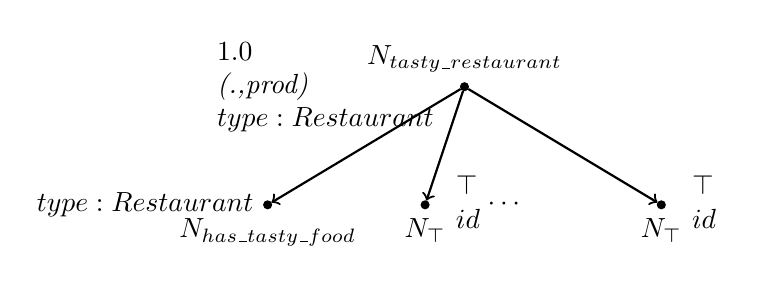
\begin{tikzpicture}[yscale=-1,
place/.style={circle,draw=black, fill=black, inner sep=0pt, 
              minimum size=1mm}]

  \node[place] (1st) at (2.5, 0) [label=above: $N_{tasty\_restaurant}$,
                                label=left: 
             \begin{tabular}{l}
               $1.0$\\
               \textit{(.,prod)}\\
               $type : Restaurant$\\
             \end{tabular}
] {};
	\node[place] (2nd) at (0, 1.5) [label=below: $N_{has\_tasty\_food}$, 
        label=left: $type : Restaurant$] {};
        \node[place] (3rd) at (2, 1.5) [label=below: $N_{\top}$,
          						  label=right: 
             \begin{tabular}{l}
            $\top$\\
            $id$\\
             \end{tabular}
             ] {}; 
        \node[place] (4rd) at (5, 1.5) [label=below: $N_{\top}$,
          						  label=right: 
             \begin{tabular}{l}
            $\top$\\
            $id$\\
             \end{tabular}
             ] {}; 

        \node (dots) at (3,1.5) {$\cdots$};
	
	\draw[->, thick] (1st) -- (2nd);
        \draw[->, thick] (1st) -- (3rd);
        \draw[->, thick] (1st) -- (4rd);
\end{tikzpicture}
\end{center}   
\caption{predicate tree for tasty\_restaurant with equivalence extension}
\label{fig:ex2.2}
\end{figure}
\end{ex}

